\begin{figure}[!b]
   \centering
   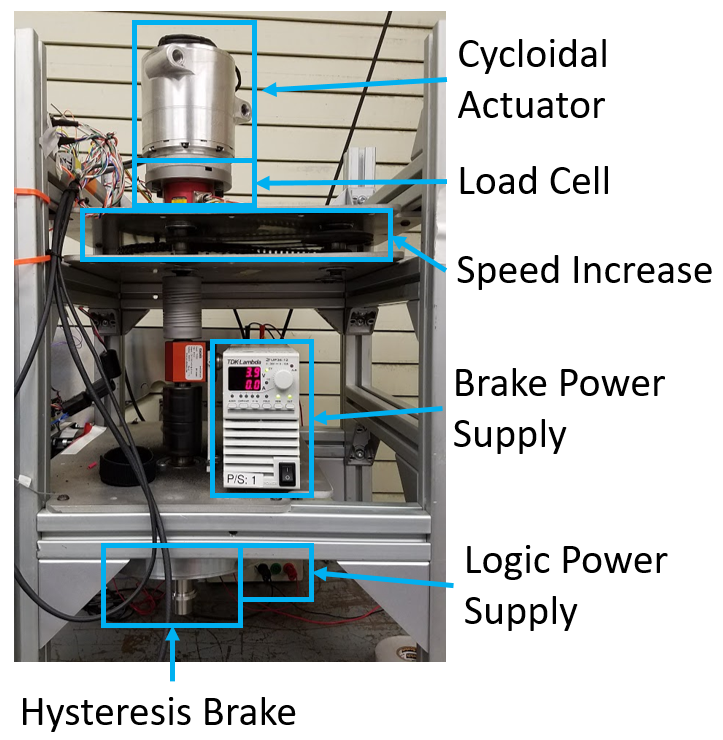
\includegraphics[width=0.75\linewidth]{images/test_stand}
   \caption{Experimental Test Setup.
   The cycloid actuator is mounted to structure via the load cell.
   There is a speed increase so the brake can generate enough torque on the system.
   Not pictured is the controlling computer, motor driver, and high voltage supply.}
   \label{test_setup}
\end{figure}

The authors sought to experimentally determine and compare the cycloidal drive in-use efficiency results to the published performance data for a comparable harmonic drive.The test setup is shown in Fig \ref{test_setup}.
The actuator is mounted directly to a Futek TF600 5000inlb load cell to measure direct output torque of the actuator.
This is read through a load cell conversion board into the motor driver.
A verification of torque readings was completed using a calibrated torque wrench to ensure accuracy of the conversion.
The motor output runs through a 36:1 (TODO) speed increase via three chain stages that then inputs into a Magtrol HB-1750 hysteresis brake that is powered using a separate 24V Lambda-TDK power supply controlled by the computer.
The motor is driven with a custom motor driver powered from a 12V Lambda-TDK power supply for logic power, and a 300V, 5A TDK-Lambda power supply for motor power.
The motor is commutated using the incremental encoder and an index pulse and is reading the RMS phase current, motor and bridge temperatures with thermistors, motor velocity, and the torque measurement from the custom conversion board.
These values are then streamed to a controlling computer that is also monitoring the high voltage supply and recording voltage and current to determine input power to the system.

Due to the tightly integrated actuator design, the motor and cycloid cannot be separated to purely isolate the losses in the cycloid.
The efficiency map of the motor over its torque and speed range was provided by Parker Motors.
For calculation purposes, this table is used as a lookup table for efficiency of the motor given the current motor velocity and rms input current.
While this does generate a level of uncertainty in the data, these motors are mass manufactured and defects are assumed to be small.
Therefore, the error in the motor efficiency map is assumed to be small and would not influence the perceived trends and results.
The efficiency losses in the motor driver can be characterized primarily by the TODO -- switching electronics and which are rated as 97\% efficient in this voltage and current range -- TODO.

\begin{figure}[!b]
   \centering
   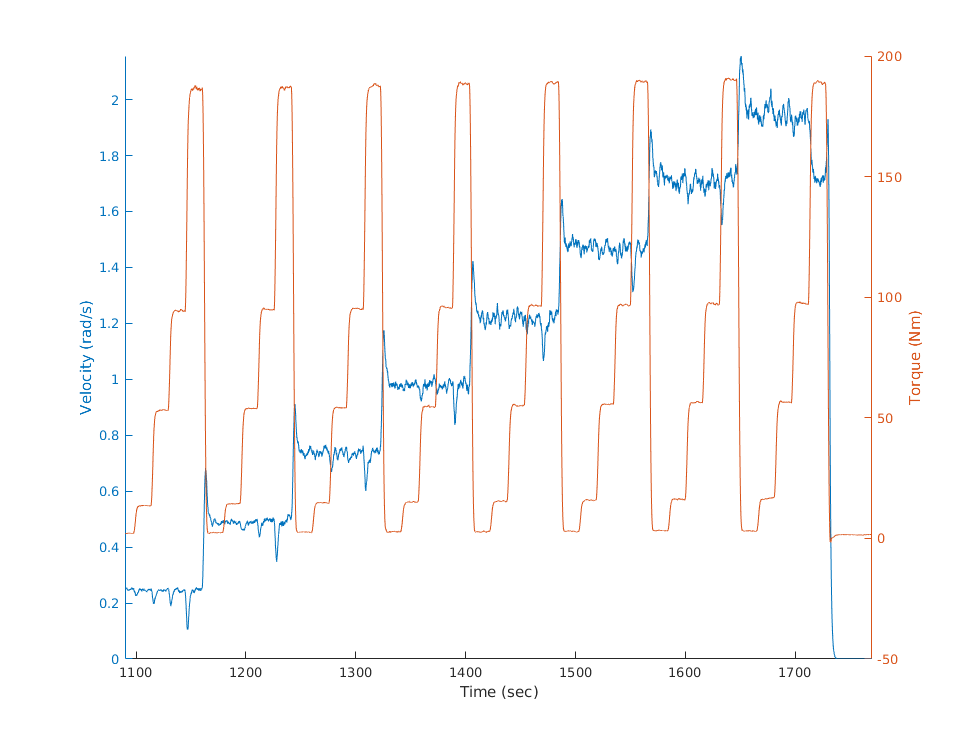
\includegraphics[width=\linewidth]{images/eff_test_profile_v3}
   \caption{Testing profile for efficiency.
   At each speed step, torque is ramped up through five different levels, then the speed is increased.
   At the last step, the maximum of the supply was reached so motor velocity dropped.}
   \label{eff_profile}
\end{figure}

The system was tested in two separate ways, an efficiency cycle and a long term drive cycle.
The efficiency cycle test was run after the long term drive cycle to ensure steady state performance before cycling through a set of velocities and torques.
The actuator is subjected to eight velocity steps increasing 0.25 rad/s each time.
In each velocity step, the torque is ramped up and maintained for 15 seconds at values of 1Nm, 15Nm, 52Nm, 94Nm, and 189Nm.
This testing profile can be seen in Fig \ref{eff_profile}.
The long term drive cycle was run continuously each day for 6 to 12 hours with the duty cycles shown in Table \ref{table_2}.
The total runtime of the system not including the initial checkout and verification of the actuator has been 111 hours.

\begin{table}[h]
  \caption{Long Run Drive Cycle}
  \label{table_2}
  \begin{center}
    \begin{tabular}{|c||c||c|}
    \hline
    Time (s) & Velocity (rad/s) & Torque (Nm)\\
    \hline
    150 & 1.0 & 0.0\\
    \hline
    150 & -1.0 & 0.0\\
    \hline
    60 & 0.5 & 26.0\\
    \hline
    60 & -0.5 & 26.0\\
    \hline
    150 & 1.5 & 10.0\\
    \hline
    150 & -1.5 & 10.0\\
    \hline
    30 & 1.0 & 50.0\\
    \hline
    30 & -1.0 & 50.0\\
    \hline
    300 & 0.5 & 18.0\\
    \hline
    300 & -0.5 & 18.0\\
    \hline
    \end{tabular}
  \end{center}
\end{table}

It should be noted that the actuator was used briefly in the robot validation after initial development and construction of the prototype wheel module.
The total time of use was approximately three hours.
Afterwards, it was removed from the wheel module and subjected to the individual testing that is discussed in this work.
The motor has a continuous current rating of 4.3 A\textsubscript{rms} and a peak rating of 15A\textsubscript{rms}.
The actuator was designed to be fluid cooled to allow operations above the continuous values, but this could not be achieved during testing.
For long duration testing, the torque values were decreased to avoid thermal issues.
The motor was tested to approximately 6A\textsubscript{rms} during efficiency testing due to the limit of the power supply.
Also, the motor driver's rated limits are 150V, therefore the actuator's maximum rated speeds could not be attained.
The nominal cycle of the actuator as seen in Fig \ref{duty_cycle} is still achievable and has been tested.

\begin{figure*}[t]
   \centering
   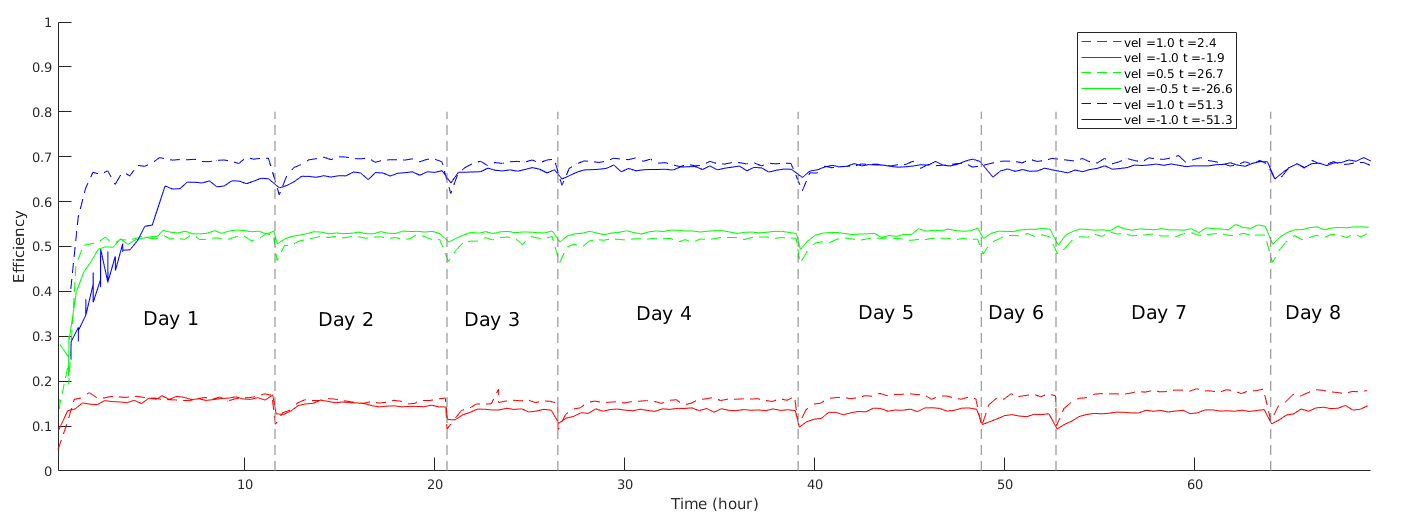
\includegraphics[width=\linewidth]{images/long_run_plot_v3}
   \caption{Efficiency over time for three different speed/torque profiles during the drive cycle.
   The forward motion can be seen with the dotted line, reverse with the solid line.
   At the onset of testing, visible efficiency gains are made.
   As each day begins, there is a clear warm-up period before steady state.
   TODO: add a line for start of each day}
   \label{long_run}
\end{figure*}

